% arara: lualatex: { shell: yes }
% arara: lualatex: { shell: yes }
\documentclass[
	spanish,
	9pt,
	xcolor=table,
	handout,
	aspectratio=1610,
	ignorenonframetext
]{beamer}

\usepackage[spanish]{babel}
\usepackage[
	cursointroductorio,
	fullpagenumbering
]{dunestyle-beamer}
\usepackage{booktabs}
\usepackage{longtable}

\usepackage[backend=biber,style=numeric, defernumbers=true, sorting=ynt,maxbibnames=4,maxcitenames=4]{biblatex}
\addbibresource{dune-doxygen-references.bib}

\title{
	Introducción a~\doxygen{}
}
\subtitle{
	Parte III:
	Uso del comando \lstinline{doxygen}
}

\author{}
\institute[]
{
	\noindent
	Practique los ejemplos en Gitpod

	\href{https://gitpod.io\#/https://github.com/cpp-review-dune/dune-basics}{
\includegraphics[width=4.5cm]{open-in-gitpod}}

	\vfill

	\begin{minipage}{0.12\paperwidth}
		Disponible en
	\end{minipage}%
	\hfill%
	\begin{minipage}{0.18\paperwidth}
		\href{https://github.com/cpp-review-dune}{
\includegraphics[width=1.2cm]{GitHub-Mark-120px-plus}}
	\end{minipage}

	\vfill

	\begin{minipage}{0.26\paperwidth}
		¡Únete al grupo en Telegram!
	\end{minipage}%
	\hfill%
	\begin{minipage}{0.04\paperwidth}
		\href{https://t.me/joinchat/OsfYP1xnFlxjN2Ix}{
\includegraphics[width=1.2cm]{telegram-logo}}
	\end{minipage}

}

\setbeamertemplate{bibliography item}{%
	\ifboolexpr{ test {\ifentrytype{book}} or test {\ifentrytype{mvbook}}
		or test {\ifentrytype{collection}} or test {\ifentrytype{mvcollection}}
		or test {\ifentrytype{reference}} or test {\ifentrytype{mvreference}} }
	{\setbeamertemplate{bibliography item}[book]}
	{\ifentrytype{online}
		{\setbeamertemplate{bibliography item}[online]}
		{\setbeamertemplate{bibliography item}[article]}}%
	\usebeamertemplate{bibliography item}}

\defbibenvironment{bibliography}
{\list{}
	{\settowidth{\labelwidth}{\usebeamertemplate{bibliography item}}%
		\setlength{\leftmargin}{\labelwidth}%
		\setlength{\labelsep}{\biblabelsep}%
		\addtolength{\leftmargin}{\labelsep}%
		\setlength{\itemsep}{\bibitemsep}%
		\setlength{\parsep}{\bibparsep}}}
{\endlist}
{\item}

\newcommand{\doxygen}{%
	\begingroup\normalfont
	
\includegraphics[height=2\fontcharht\font`B]{doxygen}%
	\endgroup
}

\begin{document}

\frame[plain,noframenumbering]{\titlepage}

\begin{frame}
	\frametitle{Objetivos de esta introdución}
	.
	\begin{itemize}
		\item .
	\end{itemize}
\end{frame}

\begin{frame}
	\frametitle{Ideas para explicar Doxygen}
	\begin{itemize}
		\item
		
		Utilizar la documentación de Doxygen.
		
		\item
		
		Explicar el uso del manual y la configuración.
	\end{itemize}
\end{frame}

\begin{frame}[fragile]\LARGE
	\begin{lstlisting}
gitpod ~/dune-basics $ tldr doxygen

doxygen
La documentación del sistema para varios lenguajes se puede encontrar en: 
	http://www.doxygen.nl.

- Para generar un archivo o plantilla de configuración utilice el comando 'Doxyfile':
	doxygen -g

- Para generar un archivo o plantilla de configuración con un nombre específico 'MiDoxygen':
	doxygen -g MiDoxygen

- Genera una plantilla de un archivo de configuración:
	doxygen -g ruta/a/archivo_de_configuracion

- Genera documentación usando un archivo de configuración existente:
	doxygen ruta/a/archivo_de_configuracion
\end{lstlisting}
\end{frame}

\begin{frame}[fragile]
	En caso de no tener instalado doxygen en Arch Linux o derivados el programa utilice el comando:\LARGE
	\begin{lstlisting}
gitpod ~/dune-basics $ yay -Sy doxygen --noconfirm
\end{lstlisting}

	\begin{lstlisting}
gitpod ~/dune-basics $ doxygen -g MiDoxigen

Configuration file 'MiDoxigen' created.

Now edit the configuration file and enter

  doxygen MiDoxigen

to generate the documentation for your project
\end{lstlisting}
\end{frame}

\begin{frame}
	El archivo \lstinline{MiDoxygen} es un archivo de texto plano con
	alrededor de $2600$ líneas, que contiene la configuración, su
	estructura es del tipo clave valor, con líneas comentadas por \#, a
	continuación explicaremos algunas de ellas para hacer una
	configuración básicas, en caso de necesitar más información dirijase
	a la página~\cite{Doxygen2021}.%\url{https://www.doxygen.nl/manual/index.html}
\end{frame}

\begin{frame}[fragile]\LARGE
	\begin{lstlisting}
# El PROJECT_NAME puede ser una palabra simple o una secuencia de palabras 
# entre comillas dobles (a menos que usted utilice Doxywizard) esto es para 
# identificar el proyecto para el que se va a generar la documentación.
# Este nombre es usado en el título de la mayoría de las páginas generadas y en pequeños otros lugares.
# El valor por defecto es: My Project, y se le puede dar el nombre de su proyecto.

PROJECT_NAME           = "Dune-project-cpp-review"
\end{lstlisting}
\end{frame}

\begin{frame}
	Si se utiliza el programa \lstinline{doxywizard} puede configurar los parámetros del archivo \lstinline{doxyfile}.

	\begin{figure}[ht!]
		\centering
		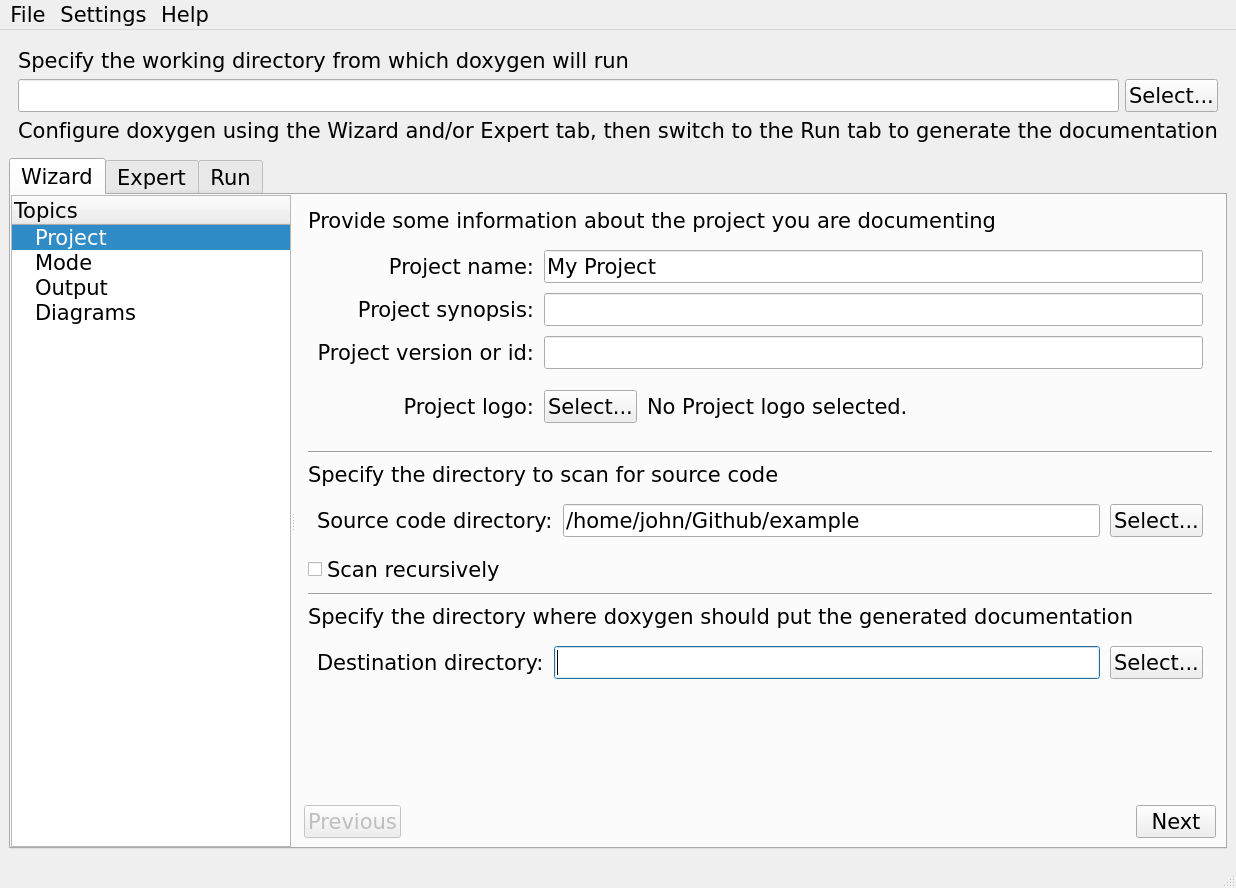
\includegraphics[scale=0.2]{wizard_capture.png}
	\end{figure}
\end{frame}

\begin{frame}[fragile]
	\frametitle{Usando doxygen con \lstinline{duneproject}}

	Una vez que ya tiene su proyecto dune configurado, automáticamente tendrá el directorio \lstinline{doc/doxygen} que con el comando \lstinline{make doxygen_dune-basics} le generará el directorio \lstinline{build/doc/doxygen/html} con la página de documentación.

	\scriptsize
	\begin{verbatim}
├── cmake
│   └── modules
│       ├── CMakeLists.txt
│       └── DuneTestMacros.cmake
├── CMakeLists.txt
├── config.h.cmake
├── doc
│   ├── CMakeLists.txt
│   └── doxygen
│       ├── CMakeLists.txt
│       └── Doxylocal
├── dune
│   ├── CMakeLists.txt
│   └── test
│       ├── CMakeLists.txt
│       └── test.hh
├── dune.module
├── dune-test.pc.in
├── README
└── src
    ├── CMakeLists.txt
    └── dune-test.cc
\end{verbatim}
\end{frame}

\begin{frame}[fragile]
	\frametitle{}
	Aeiou.
	\begin{description}
		\item[\texttt{cmake}]
		\item[\texttt{CMakeLists.txt}]
		\item[\texttt{doc}]
		\item[\texttt{dune}]
		\item[\texttt{dune.module}]
		\item[\texttt{dune-test.pc.in}]
		\item[\texttt{README}]
		\item[\texttt{src}]
	\end{description}
\end{frame}

\begin{frame}[fragile]
	El archivo \lstinline{doc/doxygen/Doxylocal} es generado luego de utilizar el comando \lstinline{duneproject}
	\begin{lstlisting}
# Este archivo contiene cambios locales en la configuración de doxygen
# por favor use '+=' para adicionar archivos/directorios a las listas

# El tag INPUT puede ser usado para espcificar los archivos y/o directorios que contienen  
# los archivos fuentes documentados.  Puede entrar archivos como "miarchivo.cpp" o
# directorios como "/usr/src/myproject".  Separe archivos o directorios con espacio.

INPUT                 += @top_srcdir@/dune/ \
                         @srcdir@/bienvenida.txt
# Vea p.ej dune-grid para ejemplos de la página principal y módulos
# INPUT                 += @srcdir@/mainpage \
#                          @srcdir@/modules

# El tag EXCLUDE puede ser usado para especificar archivos y/o directorios que deban
# ser excluidos desde los archivos fuente INPUT. De esta forma puedes fácilmente excluir un
# subdirectorio desde un árbol de directorio cuya raíz es especificado con el tag INPUT.

# EXCLUDE               += @top_srcdir@/dune/basics/test

# El tag EXAMPLE_PATH puede ser usado para especificar uno o más archivos o
# directorios que contenga fragmentos de código ejemplo que son incluidas (vea
# el comando \include).

# EXAMPLE_PATH          += @top_srcdir@/src

# El tag IMAGE_PATH puede ser usado para especificar uno o más archivos o
# directorios que contenga imagen que son incluidas en la documentación (vea
# el comando \image).

# IMAGE_PATH            += @top_srcdir@/dune/basics/pics
\end{lstlisting}
\end{frame}

\begin{frame}[fragile]
	Con Doxygen creamos un bloque de comentario en el cuerpo de una función empezando con \lstinline{/**} y ciertos parámetros señalados con el símbolo \lstinline{@} como se ve en el siguiente código
\end{frame}

\begin{frame}[fragile]
	\begin{table}[ht!]
		\caption{Comparación de la línea de comando del gestión de software (fuente: \url{wiki.archlinux.org})}
		\centering\footnotesize
		\begin{tabular}{cccp{50pt}}
			\toprule
			Acción           & Arch                  & Red Hat/Fedora          & Debian/Ubuntu
			\tabularnewline
			\midrule
			Instala paquetes & \lstinline|pacman -S| & \lstinline|dnf install| & \lstinline|apt install|
			\tabularnewline
			\tabularnewline
			\bottomrule
		\end{tabular}
	\end{table}
\end{frame}

\begin{frame}[fragile]
	\frametitle{Classes}

	\lstinputlisting[
		caption={Programa \texttt{saludo.hh}.},
		label=hello-linux.cc,
	]{../../doxygen-tutorial/src/saludo.hh}
\end{frame}

\begin{frame}\transblindsvertical
	\frametitle{Referencias}
	%------------------------------------------------------------ 1
	\only<1>{
		\begin{itemize}
			\item Libros
			      \nocite{*}
			      \printbibliography[heading=none,keyword=book]
		\end{itemize}
	}
	%------------------------------------------------------------ 2
	\only<2>{
		\begin{itemize}
			\item Artículos
			      \printbibliography[heading=none,keyword=paper]
		\end{itemize}
	}
	%------------------------------------------------------------ 3
	\only<3>{
		\begin{itemize}
			\item Sitios web
			      \printbibliography[heading=none,keyword=online]
		\end{itemize}
	}
\end{frame}

\end{document}